\section{Introduction}
\IEEEPARstart{A}{n} industrial agent that proposes a setpoint change must know which signal to read, which node to write, and which limits govern the write. On a cast-film line, for example, the agent can compare measured thickness with a production target and propose a speed adjustment. The thickness and speed signals use separate mappings even when both travel over Message Queuing Telemetry Transport (MQTT). The runtime must resolve the control node, check the caller's authority, and record what happened after the command. Fig.~\ref{fig:control-path} illustrates this sequence.

Industrial-agent research addresses service supervision, skill-based manufacturing, and fault recovery \cite{biskupovic2025supervision,koehle2026llmdriven,vyas2026detection}. Studies of programmable logic controller (PLC) integration also examine semantic grounding, approval, and proposal verification \cite{graul2026aas,schall2026safe}. We ask how one runtime can carry production context from acquisition to a governed setpoint operation when a task agent or a direct tool caller initiates the request.

We use the term \emph{production scene} for the configuration that links the line, product, recipe, and run to node mappings, drivers, objectives, and limits. The agent uses this context to select observations and propose a typed adjustment. The runtime checks the operation against live authority and limits, revalidates approved requests, and retains the command result separately from the setpoint readback and later process measurements.

The contributions are:
\begin{enumerate}
  \item A scene configuration that maps acquisition and control signals to registered drivers and supplies operating context to the runtime (Section~\ref{sec:design}).
  \item A shared dispatcher and governed operation handlers that connect agent tool calls to conditional approval, setpoint dispatch, and verification records (Sections~\ref{sec:design}--\ref{sec:modules}).
  \item An evaluation of setpoint writes and readbacks across four simulated scenes, with targeted checks of approval and guard behavior and an exploratory comparison of process trajectories under scripted writes and no-write (Section~\ref{sec:eval}).
\end{enumerate}

\begin{figure}[!b]
\centering
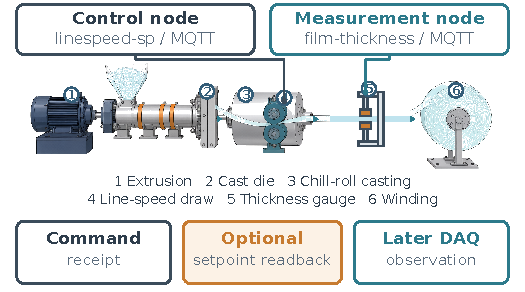
\includegraphics[width=0.98\columnwidth]{resources/fig1-vectorized-20261109.pdf}
\caption{Cast-film example. The agent reads film thickness and can propose a line-speed adjustment. The acquisition and control nodes have separate MQTT mappings. Command acceptance, setpoint readback, and later thickness measurements describe different stages of the operation.}
\label{fig:control-path}
\end{figure}


